\scanpage{51}

\uline{Lemme}\quad Soit $A$ un anneau d'endomorphismes du gpe abélien $H^*(X)$, stable par composantes homogènes (degré \uuline{total}), par transposition. \deleted{et} \inserted{Supposons $\xi\in A$, et} que pour tout $0\leq i<n$, il existe $u_i\in A$, \figure{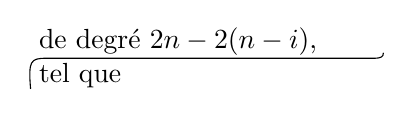
\begin{tikzpicture}[baseline=(t.base)]
\node[anchor=west,inner sep=0pt] (t) at (0,0) {tel que};
\node[anchor=south west,inner sep=0pt] at (0,0.25) {\inserted{de degré $\deleted{2n}-2(n-i)$,}};
\draw (-0.10,-0.17) .. controls (-0.13,0.19) and (-0.10,0.22) .. (0.10,0.22) -- (4.25,0.22) .. controls (4.36,0.22) and (4.38,0.24) .. (4.38,0.29);
\end{tikzpicture}}
\[
u_i\xi^{n-i}:H^i(X)\longrightarrow H^{2n-i}(X)\longrightarrow H^{i}(X)
\]
soit l'identité.
\margin{\figure{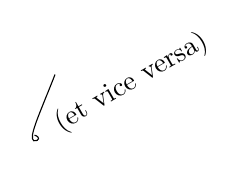
\begin{tikzpicture}[baseline=(v.base)]
\node[anchor=west,inner sep=0pt,rotate=30] (v) at (0,0) {(et vice versa)};
\draw (-0.02,0.65) .. controls (-0.22,0.14) and (-0.36,-0.15) .. (-0.29,-0.19) .. controls (-0.22,-0.20) and (-0.20,-0.14) .. (-0.28,-0.12);
\end{tikzpicture}}}
Alors $A$ contient $L$!, \deleted{les $\pi$} et les projections sur les facteurs élémentaires $\xi^jP^i$ ($i\leq n$, et \deleted{et $i+2j\leq n$ \unsure{ou} $i+2j\leq 2n-i$ \unsure{ou}} $j\leq n-i$)

\uline{Corollaire}\quad Conditions équivalentes :

(i) $L$ Algébrique

(ii) pour tt $1\leq i\unsure{<|\leq}n$, il existe une corr. \uline{alg} induisant $H^{2n-i}(X)\mathbin{-}H^i(X)$ inverse de $J^i$.

\deleted{(iii)} S'il en est ainsi, alors les \deleted{$\unsure{\xi}$} projections sur les facteurs élémentaires de $H^*(X)$, sont algébriques, et les projections $H^*(X)\mathbin{-}H^i(X)$, aussi.

\uline{Dém du lemme.}\quad Comme $A$ stable par transposition, il suffit de regarder les $\xi^jP^i$, pour $i+2j\leq n$. Soit $k=i+2j$. -- procéder par récurrence sur $k$, trivial si $k<0$.

\mspage{50}
